\documentclass[10pt,aspectratio=169]{beamer}
\usetheme{Boadilla}
\usecolortheme{dove}

\usepackage{amsmath}
\usepackage{booktabs}
\usepackage{array}
\usepackage{tikz}
\usetikzlibrary{arrows.meta,positioning}

\pdfstringdefDisableCommands{\def\translate#1{#1}}

\providecommand{\DirectionalClaimCount}{13}
\providecommand{\DirectionalIdentityCount}{10}
\providecommand{\BootstrapReplications}{1000}
\providecommand{\BootstrapBlockLength}{4}
\providecommand{\WindowInferenceStatus}{protocol defined; interval not yet estimated}


\setbeamertemplate{navigation symbols}{}
\setbeamertemplate{headline}{}
\setbeamercolor{titlelike}{parent=structure,bg=gray!10}
\setbeamercolor{item}{fg=gray!80}
\setbeamercolor{block title}{bg=gray!20,fg=black}
\setbeamercolor{block body}{bg=gray!5,fg=black}
\setbeamercolor{alertblock title}{bg=red!16,fg=black}
\setbeamercolor{alertblock body}{bg=red!4,fg=black}
\setlength{\parskip}{0pt}
\setbeamertemplate{itemize/enumerate body begin}{\vspace{-0.15em}}
\setbeamertemplate{itemize/enumerate subbody begin}{\vspace{-0.15em}}

\definecolor{pathred}{HTML}{B2182B}
\definecolor{pathblue}{HTML}{2166AC}
\definecolor{pathgreen}{HTML}{4D9221}
\definecolor{pathpurple}{HTML}{762A83}

\newcolumntype{L}[1]{>{\raggedright\arraybackslash}p{#1}}
\newcommand{\LR}{\mathrm{LR}}
\newcommand{\sourcefooter}[1]{%
  \par\vfill{\tiny\color{gray!70}Analytical source: #1}\vspace{-0.35em}}

\title[Directional long-run $\theta_t$]{Identifying the Long-Run Transformation Elasticity}
\subtitle{Unbalanced accumulation, capital composition, and regime classification}
\author{Dissertation Chapter 2}
\date{July 2026}

\setbeamertemplate{footline}{%
  \leavevmode%
  \hbox{%
  \begin{beamercolorbox}[wd=.82\paperwidth,ht=2.4ex,dp=1.1ex,leftskip=1em]{author in head/foot}%
    \insertshorttitle\hfill Directional identification correction
  \end{beamercolorbox}%
  \begin{beamercolorbox}[wd=.18\paperwidth,ht=2.4ex,dp=1.1ex,center]{date in head/foot}%
    \insertframenumber/\inserttotalframenumber
  \end{beamercolorbox}}%
}

\begin{document}

% Main 1
\begin{frame}{Long-run $\theta$ follows the unbalanced accumulation path}
  \begin{columns}[T,onlytextwidth]
    \begin{column}{0.58\textwidth}
      \begin{block}{Historical directional object}
        \centering
        \Large
        $\displaystyle
        \theta_{\Gamma,t}^{\LR}
        =
        \left.
        \frac{d\ln Y_t^p}{d\ln K_t^{cap}}
        \right|_{\Gamma^{\LR}}$
      \end{block}
      \small
      $\Gamma^{\LR}$ is the actual or estimated long-run direction in the
      $(K^{ME},K^{NR})$ capital space. The derivative therefore evaluates the
      capacity payoff of the accumulation process the economy actually follows.
    \end{column}
    \begin{column}{0.39\textwidth}
      \begin{block}{Two empirical resolutions}
        \small
        \textbf{Local:}
        $\displaystyle \theta_{\Gamma,t}=g_t^p/g_{K,t}$

        \vspace{0.7em}
        \textbf{Long-run window:}
        $\displaystyle
        \Theta_{\Gamma,w}^{\LR}
        =\frac{\sum_{t\in w}g_t^p}{\sum_{t\in w}g_{K,t}}$
      \end{block}
    \end{column}
  \end{columns}
  \begin{alertblock}{Identification verdict}
    Annual observations reveal local path slopes; the accumulation window supplies the long-run regime object. Neither requires balanced growth.
  \end{alertblock}
  \sourcefooter{A03 aggregate transformation benchmark; S33 heterogeneous-capital recovery ledger}
\end{frame}

% Main 2
\begin{frame}{Observed output still separates capacity from realized use}
  \begin{block}{Accounting separation}
    \centering
    \Large $y_t=y_t^p+\log\mu_t$
  \end{block}

  \vspace{0.5em}
  \centering
  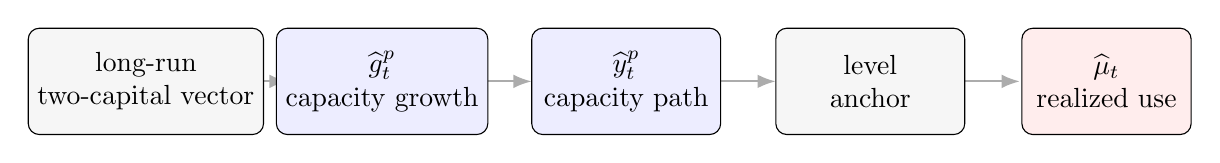
\begin{tikzpicture}[>=Latex, every node/.style={align=center}]
    \draw[->,thick,gray!65] (2.15,0) -- (2.85,0);
    \draw[->,thick,gray!65] (5.25,0) -- (5.95,0);
    \draw[->,thick,gray!65] (8.35,0) -- (9.05,0);
    \draw[->,thick,gray!65] (11.45,0) -- (12.15,0);
    \node[draw,rounded corners,fill=gray!7,minimum width=2.15cm,minimum height=1.35cm] at (1.05,0)
      {long-run\\two-capital vector};
    \node[draw,rounded corners,fill=blue!7,minimum width=2.40cm,minimum height=1.35cm] at (4.05,0)
      {$\widehat g_t^p$\\capacity growth};
    \node[draw,rounded corners,fill=blue!7,minimum width=2.40cm,minimum height=1.35cm] at (7.15,0)
      {$\widehat y_t^p$\\capacity path};
    \node[draw,rounded corners,fill=gray!7,minimum width=2.40cm,minimum height=1.35cm] at (10.25,0)
      {level\\anchor};
    \node[draw,rounded corners,fill=red!7,minimum width=2.15cm,minimum height=1.35cm] at (13.25,0)
      {$\widehat\mu_t$\\realized use};
  \end{tikzpicture}

  \vspace{0.8em}
  \begin{alertblock}{The residual remains an admissibility object}
    Residual stationarity admits the long-run capacity relation. Only the reconstructed and anchored $y_t^p$ determines the level of $\mu_t$.
  \end{alertblock}
  \sourcefooter{Binding distribution-conditioned identification sequence}
\end{frame}

% Main 3
\begin{frame}{Persistent distribution selects technique before installation}
  \begin{columns}[T,onlytextwidth]
    \begin{column}{0.57\textwidth}
      \begin{block}{Long-run technique choice}
        \centering
        $\displaystyle
        q_t^*=\arg\max_q\bigl[a(q)-q\pi_t^{\LR}\bigr]$

        \vspace{0.55em}
        \Large $a'(q_t^*)=\pi_t^{\LR}=1-\omega_t^{\LR}$
      \end{block}
      \begin{itemize}\small
        \item The persistent distributive state selects the technique before installation.
        \item The selected technique governs the ME/NR bundle of the new increment.
      \end{itemize}
    \end{column}
    \begin{column}{0.40\textwidth}
      \begin{block}{Separate the horizons}
        \centering
        $\displaystyle \omega_t=\omega_t^{\LR}+\omega_t^{SR}$
        \vspace{0.3em}

        \begin{tabular}{@{}L{0.34\linewidth}L{0.58\linewidth}@{}}
          $\omega_t^{\LR}$ & selects the technique of new accumulation \\
          \addlinespace[0.5em]
          $\omega_t^{SR}$ & changes realized output and utilization without repricing installed capacity
        \end{tabular}
      \end{block}
    \end{column}
  \end{columns}
  \begin{alertblock}{Causal implication}
    Distribution conditions the new capital increment; it cannot revalue the physical capacity of yesterday's stock.
  \end{alertblock}
  \sourcefooter{S33 technique-choice ordering and binding identification rule}
\end{frame}

% Main 4
\begin{frame}{Fixed technique does not freeze stock composition}
  \begin{columns}[T,onlytextwidth]
    \begin{column}{0.48\textwidth}
      \begin{block}{Technique fixes the marginal bundle}
        \centering
        \Large
        $\displaystyle
        \rho_t^I(q_{t-1}^*)
        =\frac{dK_t^{ME}}{dK_t^{NR}}$
      \end{block}
      \small
      The installation rule fixes the composition of the new investment increment. It does not impose the composition of the inherited stock.
    \end{column}
    \begin{column}{0.49\textwidth}
      \begin{block}{The stock ratio changes unless both coincide}
        \centering
        \Large
        $\displaystyle
        d\tau_t
        =\frac{dK_t^{ME}}{K_t^{ME}}
        -\frac{dK_t^{NR}}{K_t^{NR}}$
      \end{block}
      \small
      A fixed marginal bundle generally produces $d\tau_t\neq0$ because its ME/NR ratio differs from the stock inherited from previous installations.
    \end{column}
  \end{columns}
  \vspace{0.7em}
  \begin{alertblock}{The category error is precise}
    Fixed technique is a causal timing restriction. Fixed stock composition is a balanced-growth restriction. Treating them as equivalent removes the mechanization mechanism from the object being identified.
  \end{alertblock}
  \sourcefooter{S33 causal ordering; A03 physical composition dynamics}
\end{frame}

% Main 5
\begin{frame}{The two-capital surface separates plant and machinery payoffs}
  \begin{block}{Composition-mediated long-run differential}
    \centering
    \Large
    $\displaystyle
    d y_t^p
    =\theta^{scale}\,d k_t^{NR}
    +\theta_t^{\tau}\,d\tau_t,
    \qquad
    \tau_t=k_t^{ME}-k_t^{NR}$
  \end{block}

  \begin{block}{Equivalent component-capital representation}
    \centering
    \Large
    $\displaystyle
    d y_t^p
    =\underbrace{(\theta^{scale}-\theta_t^{\tau})}_{\theta_t^{NR}}d k_t^{NR}
    +\underbrace{\theta_t^{\tau}}_{\theta_t^{ME}}d k_t^{ME}$
  \end{block}

  \begin{columns}[T,onlytextwidth]
    \begin{column}{0.48\textwidth}
      \small\textbf{$\theta_t^{NR}$:} plant-envelope contribution to capacity formation.
    \end{column}
    \begin{column}{0.48\textwidth}
      \small\textbf{$\theta_t^{ME}$:} machinery and technique contribution to capacity formation.
    \end{column}
  \end{columns}
  \begin{alertblock}{Identification verdict}
    The decomposition does not replace aggregate $\theta$. It identifies the structural contributions from which aggregate $\theta$ is constructed along the accumulation path.
  \end{alertblock}
  \sourcefooter{Composition-mediated specification B in the binding rule and A05}
\end{frame}

% Main 6
\begin{frame}{Capital growth and potential-output growth share one path}
  \begin{columns}[T,onlytextwidth]
    \begin{column}{0.54\textwidth}
      \begin{block}{Exact capital coordinate}
        \centering
        $\displaystyle
        K_t^{cap}=K_t^{ME}+K_t^{NR}$

        \vspace{0.4em}
        $\displaystyle
        k_t^{cap}=k_t^{NR}+\ln(1+e^{\tau_t})$

        \vspace{0.4em}
        \Large
        $\displaystyle
        d k_t^{cap}=d k_t^{NR}+s_t^{ME}d\tau_t$
      \end{block}
    \end{column}
    \begin{column}{0.43\textwidth}
      \begin{block}{Different magnitudes, one movement}
        \small
        $\displaystyle g_{K,t}=\Delta\ln K_t^{cap}$

        is productive-capital growth.

        \vspace{0.7em}
        $\displaystyle g_t^p=\Delta\ln Y_t^p$

        is the potential-output response generated along that same capital movement.
      \end{block}
    \end{column}
  \end{columns}
  \begin{alertblock}{Why the distinction must remain}
    Imposing $g_t^p=g_{K,t}$ would impose $\theta=1$ by construction. The ratio compares the response with its capital-stock base; it does not introduce a second accumulation path.
  \end{alertblock}
  \sourcefooter{D10 capital identity; A03 constant-price capital aggregation}
\end{frame}

% Main 7
\begin{frame}{The accumulation direction produces aggregate $\theta$}
  \small
  \begin{block}{One capital path, two growth rates}
    \centering
    $\displaystyle
    g_t^p
    =\theta^{scale}g_t^{NR}
    +\theta_t^{\tau}(g_t^{ME}-g_t^{NR}),
    \qquad
    \theta_{\Gamma,t}
    =\frac{g_t^p}{g_{K,t}}
    =\theta^{scale}
    +\left(\theta_t^{\tau}-s_t^{ME}\theta^{scale}\right)
      \frac{d\tau_t}{d k_t^{cap}}.$
  \end{block}
  \centering
  two-capital gradient
  $\;\longrightarrow\;$ unbalanced accumulation direction
  $\;\longrightarrow\;$ aggregate $\theta_{\Gamma,t}$
  \begin{alertblock}{Balanced accumulation is only a special benchmark}
    Only when $d\tau_t=0$ does the formula reduce to $\theta^{scale}$. Along the historical unbalanced path, composition enters the elasticity tested against unity.
  \end{alertblock}
  \sourcefooter{A03 aggregate ratio; S33 component-capital bridge; v4 directional identity audit}
\end{frame}

% Main 8
\begin{frame}{Embodiment changes timing, not the accumulation direction}
  \centering
  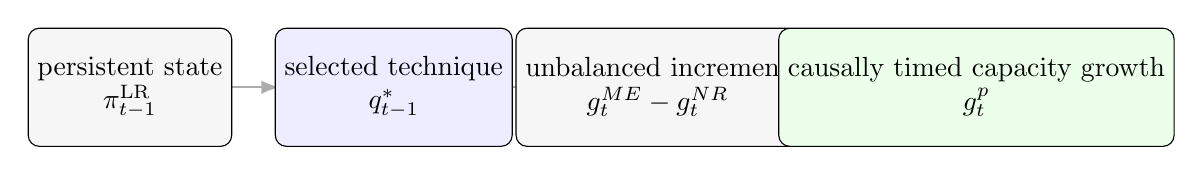
\begin{tikzpicture}[>=Latex, every node/.style={align=center}]
    \draw[->,thick,gray!65] (2.30,0) -- (3.05,0);
    \draw[->,thick,gray!65] (5.70,0) -- (6.45,0);
    \draw[->,thick,gray!65] (9.15,0) -- (9.90,0);
    \node[draw,rounded corners,fill=gray!7,minimum width=2.35cm,minimum height=1.50cm] at (1.15,0)
      {persistent state\\$\pi_{t-1}^{\LR}$};
    \node[draw,rounded corners,fill=blue!7,minimum width=2.35cm,minimum height=1.50cm] at (4.50,0)
      {selected technique\\$q_{t-1}^*$};
    \node[draw,rounded corners,fill=gray!7,minimum width=2.55cm,minimum height=1.50cm] at (7.85,0)
      {unbalanced increment\\$g_t^{ME}-g_t^{NR}$};
    \node[draw,rounded corners,fill=green!8,minimum width=3.65cm,minimum height=1.50cm] at (11.90,0)
      {causally timed capacity growth\\$g_t^p$};
  \end{tikzpicture}

  \vspace{0.8em}
  \begin{block}{Recursive capacity reconstruction}
    \centering
    \Large
    $\displaystyle
    g_t^p
    =\theta^{scale}g_t^{NR}
    +\theta_{t-1}^{\tau}(g_t^{ME}-g_t^{NR}),
    \qquad
    y_t^p=y_{t-1}^p+g_t^p$
  \end{block}
  \begin{alertblock}{Embodiment verdict}
    Lagging the technique payoff prevents current distribution from repricing installed capital. It does not suppress the ME/NR direction through which the new technique enters the stock.
  \end{alertblock}
  \sourcefooter{S33 causal order and composition-mediated Golden-Age reconstruction}
\end{frame}

% Main 9
\begin{frame}{The affine profit-share form requires composition restrictions}
  \begin{columns}[T,onlytextwidth]
    \begin{column}{0.42\textwidth}
      \begin{block}{Map the estimated wage-share state}
        \centering
        $\displaystyle \pi_t^{\LR}=1-\omega_t^{\LR}$

        \vspace{0.5em}
        $\displaystyle
        \theta_t^{\tau}
        =\psi+\lambda_\omega\widetilde\omega_{t-1}^{\LR}
        \equiv\psi_\pi+\lambda_\pi\pi_{t-1}^{\LR}$
      \end{block}
    \end{column}
    \begin{column}{0.55\textwidth}
      \begin{block}{Aggregate reduced form}
        \centering
        \small
        $\displaystyle
        \theta_{\Gamma,t}^{\LR}
        =\theta^{scale}
        +\left[
          \psi_\pi+\lambda_\pi\pi_{t-1}^{\LR}
          -s_t^{ME}\theta^{scale}
        \right]r_t^{\LR}$

        \vspace{0.45em}
        $\displaystyle
        r_t^{\LR}\equiv\frac{d\tau_t}{d k_t^{cap}}$
      \end{block}
    \end{column}
  \end{columns}
  \begin{alertblock}{The restriction must be visible}
    The governing form $\theta_t=\theta_1+\theta_2\pi_t$ follows only when $r_t^{\LR}$ and the relevant composition share are fixed over the marginal comparison, or when an explicit approximation imposes that closure. Otherwise aggregate $\theta$ remains path-dependent.
  \end{alertblock}
  \sourcefooter{Binding affine lock; composition-mediated specification; v4 methodological correction}
\end{frame}

% Main 10
\begin{frame}{Unity classifies the combined path elasticity}
  \begin{columns}[T,onlytextwidth]
    \begin{column}{0.57\textwidth}
      \begin{block}{Accumulation-window object}
        \centering
        $\displaystyle
        \Theta_{\Gamma,w}^{\LR}
        =\frac{\sum_{t\in w}g_t^p}
               {\sum_{t\in w}g_{K,t}}$

        \vspace{0.5em}
        \Large
        $\displaystyle
        \Delta_w\ln b
        =\left(\Theta_{\Gamma,w}^{\LR}-1\right)
         \Delta_w\ln K^{cap}$
      \end{block}
      \small Conditional on $\sum_{t\in w}g_{K,t}>0$:
      \begin{itemize}
        \item $\Theta_{\Gamma,w}^{\LR}<1$: capital grows faster than the capacity it builds;
        \item $\Theta_{\Gamma,w}^{\LR}=1$: capacity productivity is unchanged;
        \item $\Theta_{\Gamma,w}^{\LR}>1$: capacity grows more than proportionally.
      \end{itemize}
    \end{column}
    \begin{column}{0.40\textwidth}
      \centering
      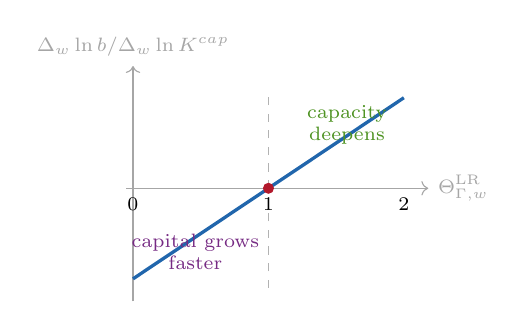
\begin{tikzpicture}[x=1.72cm,y=1.15cm,font=\scriptsize]
        \draw[->,gray!70] (-0.05,0) -- (2.18,0) node[right] {$\Theta_{\Gamma,w}^{\LR}$};
        \draw[->,gray!70] (0,-1.25) -- (0,1.35) node[above] {$\Delta_w\ln b/\Delta_w\ln K^{cap}$};
        \draw[very thick,pathblue] (0,-1) -- (2,1);
        \draw[dashed,gray!60] (1,-1.1) -- (1,1.1);
        \fill[pathred] (1,0) circle (2pt);
        \node[below] at (0,0) {$0$};
        \node[below] at (1,0) {$1$};
        \node[below] at (2,0) {$2$};
        \node[align=center,pathpurple] at (0.46,-0.70) {capital grows\\faster};
        \node[align=center,pathgreen] at (1.58,0.70) {capacity\\deepens};
      \end{tikzpicture}
      \begin{alertblock}{Window rule}
        Contraction years enter the cumulative path; classification requires positive cumulative capital growth for the window.
      \end{alertblock}
    \end{column}
  \end{columns}
  \sourcefooter{Harrodian accounting identity and A03 aggregate transformation object}
\end{frame}

% Main 11
\begin{frame}{Regimes require windows; realized use still requires $\mu$}
  \scriptsize
  \renewcommand{\arraystretch}{1.12}
  \begin{tabular}{@{}L{0.25\textwidth}L{0.28\textwidth}L{0.39\textwidth}@{}}
    \toprule
    \textbf{Window interval} & \textbf{Accumulation verdict} & \textbf{Interpretive boundary} \\
    \midrule
    $U_w^{\Theta}<1$ & below-one capital-overaccumulation tendency & capital expands faster than the potential capacity it produces \\
    $L_w^{\Theta}\leq1\leq U_w^{\Theta}$ & indeterminate & the data do not identify a side of the Harrodian benchmark \\
    $L_w^{\Theta}>1$ & above-one capacity-deepening tendency & excess productive capacity additionally requires unused or increasingly unused capacity \\
    \bottomrule
  \end{tabular}

  \vspace{0.25em}
  \begin{block}{Utilization after path reconstruction}
    \centering
    \large
    $\displaystyle
    \Delta\ln\mu_t
    =\Delta y_t-g_t^p
    =\Delta y_t-\theta_{\Gamma,t}g_{K,t}$
  \end{block}
  \begin{alertblock}{Final analytical verdict}
    $\Theta_{\Gamma,w}^{\LR}$ classifies capacity creation. Anchored $\mu_t$ determines its use: above-one capacity deepening becomes excess productive capacity only when realization fails.
  \end{alertblock}
  \sourcefooter{Constitutional productive-capacity corridor; binding capacity-utilization sequence}
\end{frame}

\appendix

% Appendix 1
\begin{frame}{A1. Identification fails when any path gate fails}
  \scriptsize
  \renewcommand{\arraystretch}{1.28}
  \begin{tabular}{@{}L{0.17\textwidth}L{0.40\textwidth}L{0.35\textwidth}@{}}
    \toprule
    \textbf{Gate} & \textbf{Pass condition} & \textbf{Failure classification} \\
    \midrule
    state order & $k_t^{NR}$, $\tau_t$, and distributive conditioning are admissible long-run objects & mixed-order or polynomial-risk specification \\
    rank & scale and composition effects are separately identified & mechanization collapses into the scale direction \\
    residual & $\widehat\varepsilon_t\sim I(0)$ & no stable long-run capacity surface \\
    timing & lagged persistent distribution weights the new ME/NR increment & contemporaneous repricing of installed capacity \\
    aggregation & $K_t^{cap}=K_t^{ME}+K_t^{NR}$ and the growth denominator is reproduced & capital-path denominator is incoherent \\
    anchoring & one explicit benchmark fixes the level of $y_t^p$ & $\mu_t$ remains underidentified \\
    accumulation & $\sum_{t\in w}g_{K,t}>0$ & unity has no threshold interpretation for the window \\
    inference & the interval for $\Theta_{\Gamma,w}^{\LR}$ is economically admissible & no structural regime verdict \\
    \bottomrule
  \end{tabular}
  \vspace{0.65em}
  \begin{alertblock}{Rank has an economic meaning}
    The data must contain independent variation in plant-envelope scale and ME/NR composition. Without it, the gradient cannot be separated and the path elasticity cannot be structurally decomposed.
  \end{alertblock}
  \sourcefooter{Binding specification fork; A03/A05 measurement and promotion gates}
\end{frame}

% Appendix 2
\begin{frame}{A2. Inference must rebuild the entire unbalanced path}
  \centering
  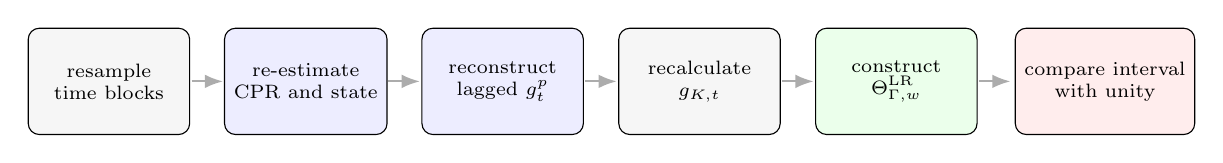
\begin{tikzpicture}[>=Latex, every node/.style={align=center,font=\scriptsize}]
    \draw[->,thick,gray!65] (2.05,0) -- (2.45,0);
    \draw[->,thick,gray!65] (4.55,0) -- (4.95,0);
    \draw[->,thick,gray!65] (7.05,0) -- (7.45,0);
    \draw[->,thick,gray!65] (9.55,0) -- (9.95,0);
    \draw[->,thick,gray!65] (12.05,0) -- (12.45,0);
    \node[draw,rounded corners,fill=gray!7,minimum width=2.05cm,minimum height=1.35cm] at (1.00,0)
      {resample\\time blocks};
    \node[draw,rounded corners,fill=blue!7,minimum width=2.05cm,minimum height=1.35cm] at (3.50,0)
      {re-estimate\\CPR and state};
    \node[draw,rounded corners,fill=blue!7,minimum width=2.05cm,minimum height=1.35cm] at (6.00,0)
      {reconstruct\\lagged $g_t^p$};
    \node[draw,rounded corners,fill=gray!7,minimum width=2.05cm,minimum height=1.35cm] at (8.50,0)
      {recalculate\\$g_{K,t}$};
    \node[draw,rounded corners,fill=green!8,minimum width=2.05cm,minimum height=1.35cm] at (11.00,0)
      {construct\\$\Theta_{\Gamma,w}^{\LR}$};
    \node[draw,rounded corners,fill=red!7,minimum width=2.25cm,minimum height=1.35cm] at (13.65,0)
      {compare interval\\with unity};
  \end{tikzpicture}

  \vspace{0.8em}
  \begin{columns}[T,onlytextwidth]
    \begin{column}{0.47\textwidth}
      \begin{block}{Required protocol}
        \BootstrapReplications\ moving-block draws with block length \BootstrapBlockLength\ years. Every draw re-estimates the coefficient and generated-state chain.
      \end{block}
    \end{column}
    \begin{column}{0.50\textwidth}
      \begin{alertblock}{Current inference status}
        \WindowInferenceStatus. The existing roughness-attribution bootstrap is not a regime interval, so this deck makes no numerical historical regime claim.
      \end{alertblock}
    \end{column}
  \end{columns}
  \sourcefooter{Required generated-state inference; \DirectionalClaimCount\ claims and \DirectionalIdentityCount\ identities validated}
\end{frame}

\end{document}
